
Il mio compito nello sviluppo dell'applicazione è stato quello 
di creare un prototipo iniziale avendo a disposizione un mock up creato con
proto.io\cite{protoio} e una serie di requisiti essenziali.

\section{Requisiti essenziali}

La base di partenza di QIX sono state delle funzionalità essenziali e 
sonstanzialmente molto difficili da inserire in una versione dell'app già avanzata.
È stati quindi deciso di creare un prototipo di partenza avente i seguenti requisiti:

\begin{itemize}
    \item {
        \textbf{Navigazione dinamica}: L'applicazione deve gestire dei cambiamenti di contesto
        dinamici: dev'essere possibile mostrare all'utente contenuti dinamici indipendentemente
        dal contesto in cui si trova.
    }
    \item {
        \textbf{QIX Shake}: L'utente deve poter agitare lo smartphone in qualsiasi
        sezione dell'applicazione e il risultato deve essere basato sul contesto attuale o su delle direttive dettate
        da delle Rest API;
    } 
    \item {
        \textbf{Animazioni interattive}: L'intera applicazione dev'essere progettata in modo tale da presentare all'utente
        delle \textbf{animazioni interattive} in stile CardView\cite{cardview} disponibili in 
        qualunque sezione o vista in cui si trovi l'utente e definite dal contesto attuale;

        Le animazioni in questione devono essere progettate in pagine, in cui ogni pagina può contenere 
        più CardView. L'utente vedrà in un determinato momento una e soltanto una pagina.

        Ogni CardView deve essere trascinabile dall'utente e deve interagire con le altre CardView della pagine. 
        Quando l'utente usa una forza di trascinamento superiore a un valore di soglia tutte le viste devono
        cadere per gravità;
        
        Tale gravità finirà con la fine dell'animazione o l'apparizione di una nuova pagina se presente;
    }
    \item {
        \textbf{Autenticazione}: L'applicazione deve supportare tre diversi stati o modalità di autenticazione:
        \begin{enumerate}
            \item\textbf{Trial Mode}: l'utente è anonimo, esiste solo un id per tenere traccia dei suoi QIX coins.
            \item\textbf{Signed Mode}: l'utente ha inserito il numero di telefono e il suo genere;
            \item \textbf{Pro Mode}: l'utente aggiunge dei dati su se stesso o collega il suo account a dei social media come Facebook, Google o Instagram;
        \end{enumerate}
        Si nota facilmente che non esiste una stato in cui l'utente non è registrato: questo perchè
        per tenere traccia dei suoi QIX coins e di altri dati utili è necessario avere una riferimento all'utente;
    }
    \item {
        \textbf{DeepLinks}: L'applicazione deve poter essere avviata dinamicamente
        attraverso dei \textbf{Deep Links}\cite{deeplinks};
        E deve essere in grado di gestirli in base al contesto dell'utente;
    }
\end{itemize}

\section{La navigazione dinamica}

% Analizzando il requisito mi sono posto diverse domande: \\ \\
% \noindent{
%     \large\textit{Cosa significa dinamicamente?}
%     \normalsize{Il nostro obiettivo in questo caso è mostrare all'utente \textbf{contenuti diversi}
%     indipendentemente dal constesto e quindi dalla vista in cui si trova}\\ \\
%     \large\textit{Quale contesto?}
%     \normalsize{Con contesto dell'utente si intende lo stato attuale dell'applicazione,
%     quindi l'intero stack di navigazione se presente;
%     } \\ \\
% }

Prima di entrare nel merito della soluzione al problema, elenco brevemente gli
standard di navigazione delle app iOS.

Ogni applicazione può avere degli \textbf{UINavigationController}\cite{navigationcontroller},
ossia dei contenitori di \textbf{UIViewController}\cite{viewcontroller} che vengono
utilizzati per mantenere lo stack di navigazione e gestire la transizioni tra due UIViewController.

Nella figura~\ref{fig:1} si nota facilmente come il Navigation controller gestisce un'array di View Controller e una sola 
navigation bar. 
In iOS sono infatti innate molte animazioni di navigazione che è utile sfruttare, piuttosto di creare 
componenti custom poi difficili da rendere interattivi.\\

\begin{minipage}{\linewidth}
    \centering
    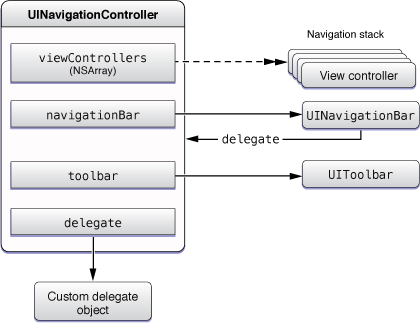
\includegraphics[width=5cm]{navigation}
    \captionof{figure}{Navigation controller scheme}
    \label{fig:1}
\end{minipage}

\subsection{Tipologie di navigazione}\label{sec:navigation}

Esistono tre tipologie base di navigazione:

\begin{enumerate}
    \item{\textbf{Push}: un UIViewController avente un navigation controller può rendere
    visibile un altro ViewController attraverso la funzione "pushViewController" di un Navigation controller\par
    \begin{minipage}{\linewidth}
        \centering
        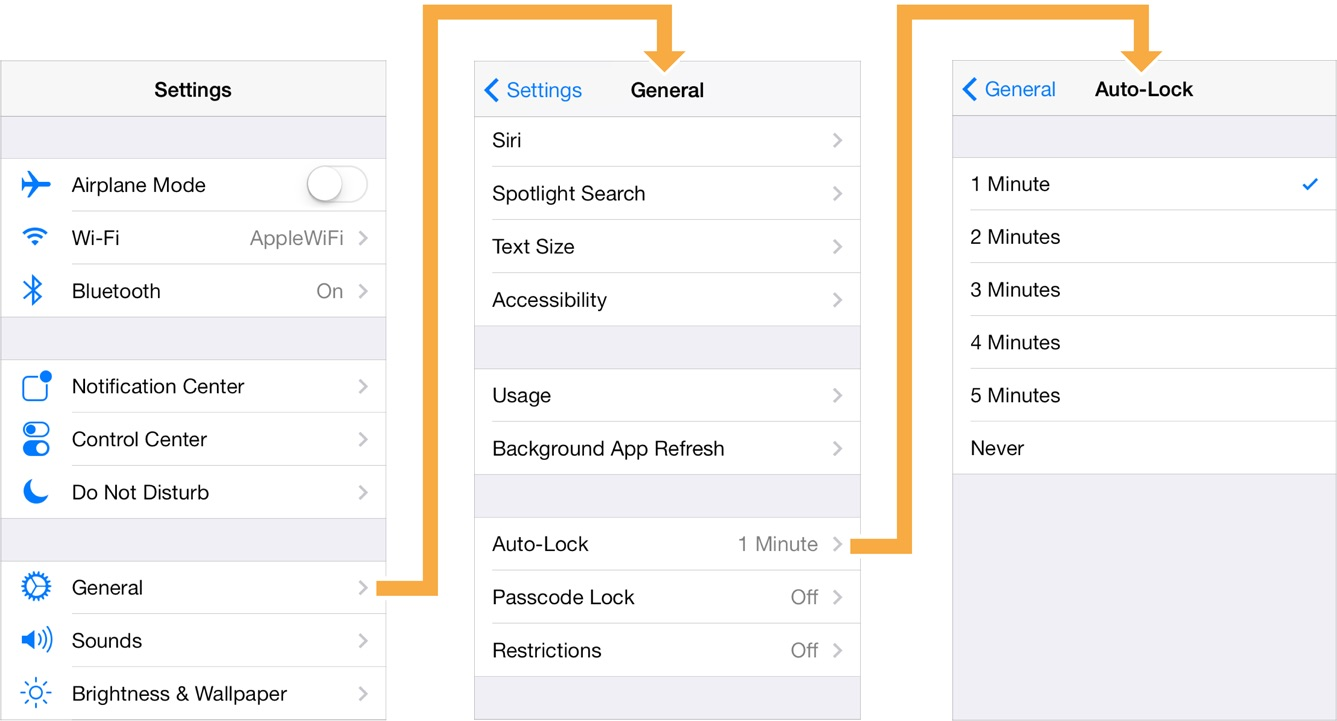
\includegraphics[width=10cm]{push}
        \captionof{figure}{Presantazione di un ViewController tramite push}
        \label{fig:2}
    \end{minipage}
    }
    \item{ \textbf{Modal}: un ViewController può presentare un altro ViewController senza necessariamente avere un 
        Navigation Controller, l'animazione standard è dal basso verso l'alto come in figura~\ref{fig:3}\par
        \begin{minipage}{\linewidth}
            \centering
            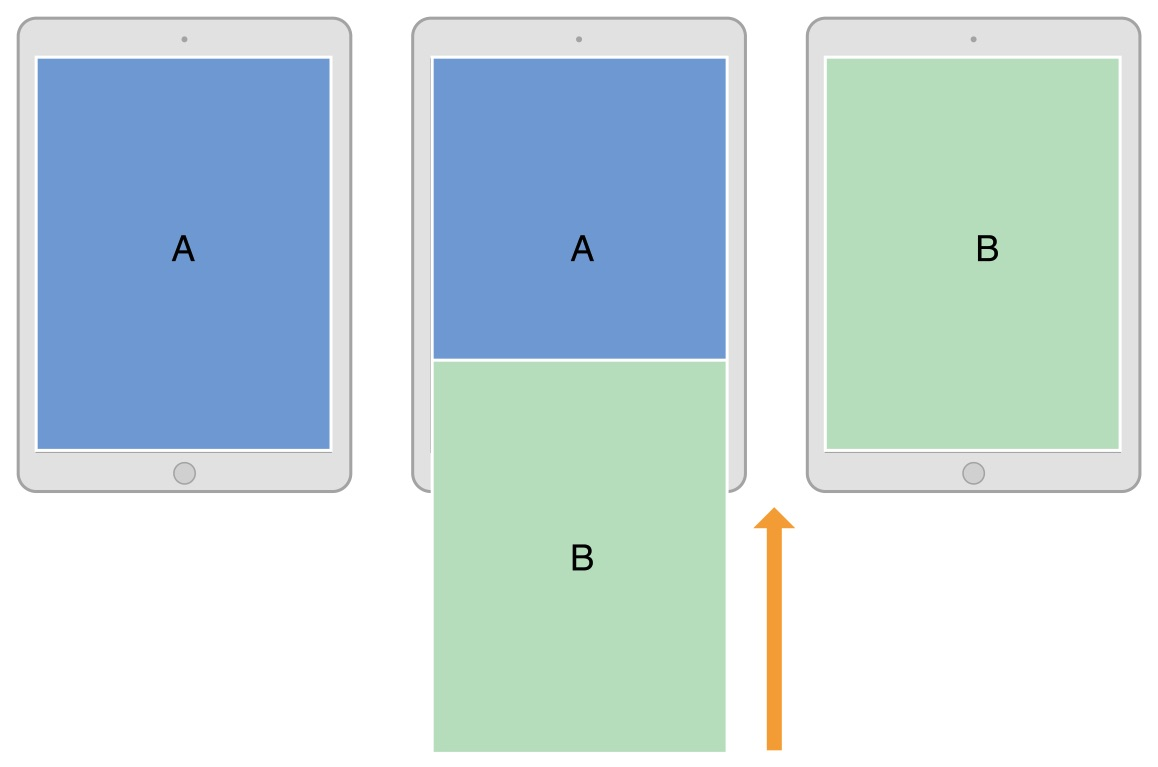
\includegraphics[width=10cm]{modal}
            \captionof{figure}{
                Presantazione di un ViewController tramite modal
            }
            \label{fig:3}
        \end{minipage}
    }
    \item{\textbf{Segue}: Una segue non è altro che un link tra due view controller attraverso un'interfaccia
        grafica. In base alla tipologia cambia il tipo di navigazione (Modal o Push)
    }
\end{enumerate}

Avendo definito i principali metodi di navigatione tra ViewController torniamo al problema iniziale:
\textit{Come possiamo rendere dinamica la navigazione?}

A seguito di uno studio approfondito di varie tecniche di navigazione iOS ho scelto di utilizzare il
\textbf{Coordinator Pattern}\cite{coordinatorpattern}.

\subsection{Il Coordinator Pattern}

Generalmente in iOS l'intera logica di un ViewController viene scritta nel ViewController stesso, creando spesso
file di grosse dimensioni e disordine generale. Il Coordinator Pattern è nato proprio per rendere 
le applicazioni più scalabili e leggere. 

Ogni ViewController infatti delega tutte le decisioni al suo Coordinator che in base a determinate logiche deciderà
i passi successivi.

Ogni Coordinator può controllare un ViewController o più Coordinator, questo rende le viste
indipendenti tra di loro e rende ogni ViewControler totalmente invisibile agli altri.\\

\begin{minipage}{\linewidth}
    \centering
    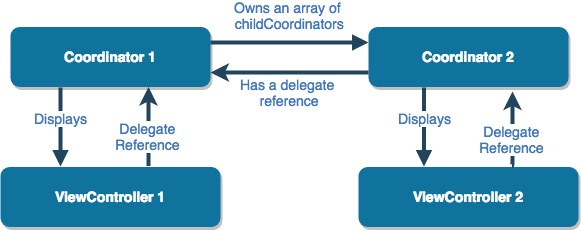
\includegraphics[width=10cm]{coordinator}
    \captionof{figure}{
        Il Coordinator Pattern
    }
    \label{fig:4}
\end{minipage}\\ \\

La resposibilità dei coordinator è infatti la navigazione, come un navigation controller gestisce i sui View Controller, un coordinator gestisce
i suoi figli e questo rende ogni vista o flow di navigazione totalmente indipendente dal resto dell'applicazione.

Per navigare tra i view controller vengono generalmente usate le tipologie di navigazione
descritte nella sezione~\ref{sec:navigation}, tranne le segue, che essendo definete da vista grafica renderebbero
la navigazine statica e fissata su determinati ViewController. \\

Di seguito in figura~\ref{fig:5} presento uno schema dell'utilizzo di due coordinator
per la gestione di una lista di prodotti e il carrello. \\

\begin{minipage}{\linewidth}
    \centering
    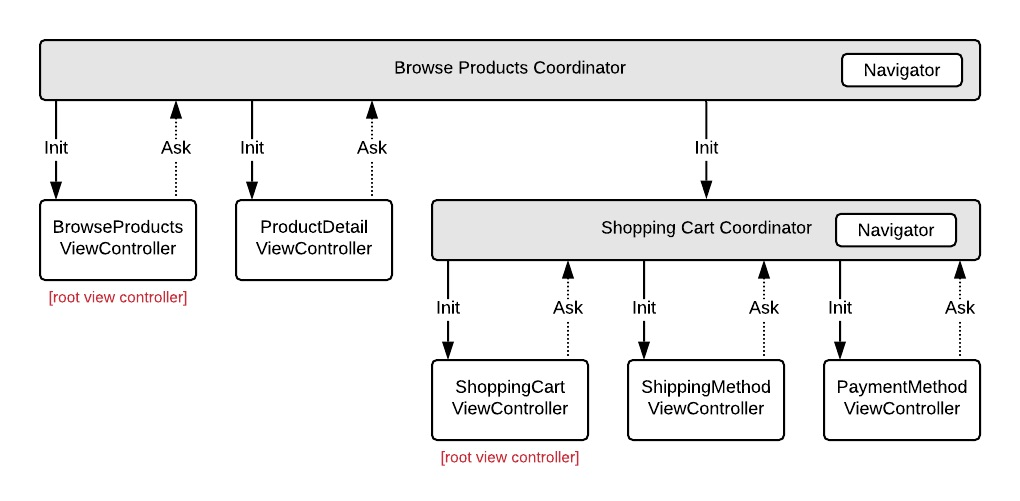
\includegraphics[width=10cm]{coordinator-example}
    \captionof{figure}{
       Esempio di coordinator pattern
    }
    \label{fig:5}
\end{minipage}\\ \\

Come si evince dall'immagine è presente in entrambi i coordinator è presente un oggetto
\textbf{navigator} che sarà in gestore di un UINavigationController

\section{Il QIX Shake}

In iOS ogni UIViewController risponde a degli eventi. L'evento designato per lo shake è
\begin{minted}{swift}
    func motionEnded(_ motion: UIEvent.EventSubtype,
        with event: UIEvent?)
\end{minted}

In caso di shake infatto motion sarà uguale a .motionShake
Per rendere disponibile l'evento "shake" in un qualunque ViewController la soluzione è stata abbastanza semplice:
è bastato l'utlizzo di un ViewController Genitore e attrvaerso l'eriditarietà ogni view controller è in grado
di eseguire la stessa funzionalità.

In questo caso è stato optato l'utilizzo delle notifiche locali: quando avviene uno shake i view controller inviano una notifica 
globale e solo gli observer vi hanno accesso.

\section{Le animazioni interattive}

Per semplicità divido il requisito in diversi punti e per ognuno ne spiego la soluzione
o metodologia utilizzata:

\begin{enumerate}
    \item\label{animationenum:1} Le animazioni devono essere disponibili in qualunque sezione o vista in cui si trovi l'utente e definite dal contesto attuale;

    \item\label{animationenum:2} Ogni CardView deve essere trascinabile dall'utente;
    
    \item\label{animationenum:3} Quando l'utente usa una forza di trascinamento superiore a un valore di soglia tutte le viste devono
        cadere per gravità;

    \item\label{animationenum:4} Le animazioni in questione devono essere progettate in pagine, in cui ogni pagina può contenere 
    più CardView. L'utente vedrà in un determinato momento una e soltanto una pagina;

    \item\label{animationenum:5} Una volta che le animazione acquisisco una gravità e cadono, finirà l'animazione o l'apparirà
    una nuova pagina se presente;

    \item\label{animationenum:6} Ogni CardView deve interagire con le altre della stessa pagina, come se si toccassero;

\end{enumerate}

% % % % % % % % % % % % % % % % % % % % % % % % % % % % % % % % % % % % %
%                      Onnipresenza delle animazioni                    %
% % % % % % % % % % % % % % % % % % % % % % % % % % % % % % % % % % % % %
\subsection{~\ref{animationenum:1}. Onnipresenza delle animazioni}

\textbf{Premessa}: il contenuto di ogni applicazione iOS è inserito all'interno di un oggetto denominato
    \textbf{UIWindow}\cite{uiwindow}. Questa finistra è disponibile in ogni UIViewController e permette di aggiungere contenuti
    come viste o interi UIViewController al di sopra di tutto il contesto dell'app. Questo rende essenzialmente ogni contenuto presentato
    indipendente per esempio da un stack di navigazione.\\ 

Per creare animazioni definite dal contesto usiamo quindi un semplice UIViewController che gestirà tutte le animazioni,
ma invece di presentarlo attraverso i metodi base visti alla sezione~\ref{sec:navigation}, lo presentiamo al di sopra della UIWindow,
in modo da non essere vincolati dal contesto dell'utente quando l'animazione finirà.

% % % % % % % % % % % % % % % % % % % % % % % % % % % % % % % % % % % % %
%                        CardView trascinabile                          %
% % % % % % % % % % % % % % % % % % % % % % % % % % % % % % % % % % % % %
\subsection{~\ref{animationenum:2}. Aggiunta di una gesture}

In iOS per interagire con le viste attraverso il display touch screen si utilizzano delle UIGestureRecognizer.
Tali strumenti sono nativi e offrono diverse tipologie per l'iterazione:
\begin{itemize}
    \item UITapGestureRecognizer: respansabile della gestione dei tap

    \item UIPinchGestureRecognizer: respansabile della gestione del pitch ossia la gesture spesso usata per lo zoom
    
    \item UIRotationGestureRecognizer: respansabile della gestione delle rotazioni
    
    \item UISwipeGestureRecognizer: responsabile di uno swipe ossia un trascinamento in una direzione molto breve
    
    \item UIPanGestureRecognizer: responsabile del drag and drop
    
    \item UIScreenEdgePanGestureRecognizer: responsabile di uno swipe ossia un trascinamento nei bordi dello schermo
    
    \item UILongPressGestureRecognizer: responsabile di una prossione prolungata nel tempo
\end{itemize}

Per un'animazione che deve muoversi come se l'utente la stesse spostando occore una UIPanGestureRecognizer.
In particolare una per ogni vista "draggabile".

% % % % % % % % % % % % % % % % % % % % % % % % % % % % % % % % % % % % %
%                        Gravità                                        %
% % % % % % % % % % % % % % % % % % % % % % % % % % % % % % % % % % % % %
\subsection{~\ref{animationenum:3}. Inserimento della fisica}

Per strutturare le animazioni è stato fatto un attento studio a metodologie e frameworks
atti a creare animazioni interattive fluide.

Alla fine è stato deciso di utilizzare in pacchetto
nativo di iOS incluso nello UIKit\cite{uikit}, chiamato UIKitDynamics\cite{uidynamics}: questo framework, con una serie di API 
plug and play, offre delle funzioni di animazione base che includo la fisica del mondo reale.

% % % % % % % % % % % % % % % % % % % % % % % % % % % % % % % % % % % % %
%                        Pagination                                     %
% % % % % % % % % % % % % % % % % % % % % % % % % % % % % % % % % % % % %
\subsection{~\ref{animationenum:4}. La paginazione}

% % % % % % % % % % % % % % % % % % % % % % % % % % % % % % % % % % % % %
%                   La paginazione delle animazioni                     %
% % % % % % % % % % % % % % % % % % % % % % % % % % % % % % % % % % % % %
\subsection{~\ref{animationenum:5}. Paginazione delle animazioni}

Avendo definito al punto precedente l'utilizzo di un solo UIViewController per le animazioni da un lato semplifica
la presentazione delle animazioni, dato che basterà presentare un solo ViewController, ma dall'altro delega
la paginagione al view controller. \\

L'idea di base è animare delle UIView, ossia dei rettangoli con all'interno del contenuto, per questo 

% % % % % % % % % % % % % % % % % % % % % % % % % % % % % % % % % % % % %
%                   La paginazione delle animazioni                     %
% % % % % % % % % % % % % % % % % % % % % % % % % % % % % % % % % % % % %
\subsection{~\ref{animationenum:6}. Il Collider}
